\documentclass{mc2015}

%%%%%%%%%%%%%%%%%%%%%%%%%%%%%%%%%%%%%%%%%%%%%%%%%%%%%%%%%%%%%%%%%%%%%
\usepackage[T1]{fontenc}         % Use T1 encoding instead of OT1
\usepackage[utf8]{inputenc}      % Use UTF8 input encoding
\usepackage{microtype}           % Improve typography
\usepackage{booktabs}            % Publication quality tables
\usepackage{amsmath}
\usepackage{graphicx}
\usepackage{float}
\usepackage[exponent-product=\cdot]{siunitx}
\usepackage[colorlinks,breaklinks]{hyperref}
\hypersetup{linkcolor=black, citecolor=black, urlcolor=black}

\usepackage{lipsum}

\def\equationautorefname{Eq.}
\def\figureautorefname{Fig.}

%%%%%%%%%%%%%%%%%%%%%%%%%%%%%%%%%%%%%%%%%%%%%%%%%%%%%%%%%%%%%%%%%%%%%
% Insert authors' names and short version of title in lines below

\authorHead{Chris Dances, Vince Mousseau, Maria Avramova}
\shortTitle{Transient Verification of COBRA-TF}

%%%%%%%%%%%%%%%%%%%%%%%%%%%%%%%%%%%%%%%%%%%%%%%%%%%%%%%%%%%%%%%%%%%%%
\begin{document}

\title{Initial 1-D Single Phase Liquid Transient Verification of COBRA-TF}

\author{Chris Dances}
\author{Dr. Maria Avramova}
\affil{ Department of Mechanical and Nuclear Engineering \\
  The Pennsylvania State University \\
  137 Reber Building, University Park, PA, 16802, USA \\
  cad39@psu.edu; mna109@psu.edu}

\author{Dr. Vince Mousseau}
\affil{ Computer Science Research Institute \\
  Sandia National Laboratories \\
  1450 Innovation Parkway, Albuquerque, NM 87123, USA \\
  vamouss@sandia.gov
}

\maketitle

\begin{abstract}
Abstract \ldots

\emph{Key Words}: List no more than five key words
\end{abstract}

\clearpage
%%%%%%%%%%%%%%%%%%%%%%%%%%%%%%%%%%%%%%%%%%%%%%%%%%%%%%%%%%%%%%%%%%%%%

%\tableofcontents
%\clearpage
%
%\listoffigures
%\clearpage

%%%%%%%%%%%%%%%%%%%%%%%%%%%%%%%%%%%%%%%%%%%%%%%%%%%%%%%%%%%%%%%%%%%%%
\section{Introduction}

For the past several decades, the primary focus in nuclear engineering within
the United States has been focused on light water reactors (LWR). Commercially,
all nuclear reactors are either boiling water reactors (BWR) or pressurized
water reactors (PWR). Correct computation of the thermal hydraulics within the
reactor core leads to effi- cient design and accuracy in the safety analysis. A
popular subchannel code for modelling the hydrodynamics with in the reactor core
is COBRA-TF. This FORTRAN based code solves 8 conservation equations for liquid,
entrained droplet, and vapor phases in 3-D dimmensions \cite{CTF_Theory}. A 1-D
residual formulation of the code has been created. This paper outlines an
intitial verification of the original verion of code as well as the residual
version of the code. The verification problem is a single pahes 1-D channel with
transient inlet density and mass flow rate. The problem will undergo a
Richardson's extrapolation in the temporal and spatial domains to verify the
convergence and order of accuracy of the error. The study of the order of
accuracy is considered one of the more rigourous verification criteria
\cite{VV_review}.

\section{COBRA-TF}

The thermal hydraulics of a LWR core is an important part of nuclear
reactor desigin. COBRA-TF solves 8 conservation equations for liquid,
entrained droplet, and vapor phases of water boiling within the rod structure
of a LWR reactor core \cite{CTF_Theory}. Currently, the conservation
equations analytically reduce into a pressure matrix in a semi-implicit
method with rod temperatures solved for explicitly. This work involves
representing the 1-D single phase liquid conservation equations and calculated 
variables in a residual formulation. This residual formulation should allow for
easier and more in depth verification analysis. This paper details the intitial
comparison of the residual formulation to the original code.

\subsection{Software Quality Assurance}

Software quality assurance is a set of tools and procedures that helps
ensure that the software is reliable. COBRA-TF is managed by Github repository
setup and maintained by CASL. An exensive test matrix is run before each major
push to ensure that the code meets the specificed requirements. The test matrix
consists of unit tests, code coverage runs, validation problems, and validation
problems. The code documentation consists of a theory manual, a users manual, a
developers manual, and a validation manual. Further work might involve using
autodocumentation tools to keep an up to date developers manual. This paper will
be the begining of a verification manual, integrating this verificaiton problem
directly into the test matrix.

\subsection{1-D Single Phase Liquid Conservation Equations}

The finite volume structure in COBRA-TF in figure \ref{fig:CTF-Cells} is for a
one-dimmensional channel in the axial direction with n number of cells. The
first and last cells at 0 and n + 1 are ghost cells and act as the boundary
conditions for the problem. Pressure, enthalpy, and density are averaged over
the cell volume and are located at the center of the cell. Mass flow rate and
velocity are located at the faces in between cells. The cells  are represented
with an index i, and the faces with indexes of $i + \frac{1}{2}$ or 
$i-\frac{1}{2}$. This project will initially focus on this 1-D configuration.
Usually the code  is 3-D,  with channels connecting to each other in two more 
dimmensions.

\begin{figure}[!h]
	\centering
	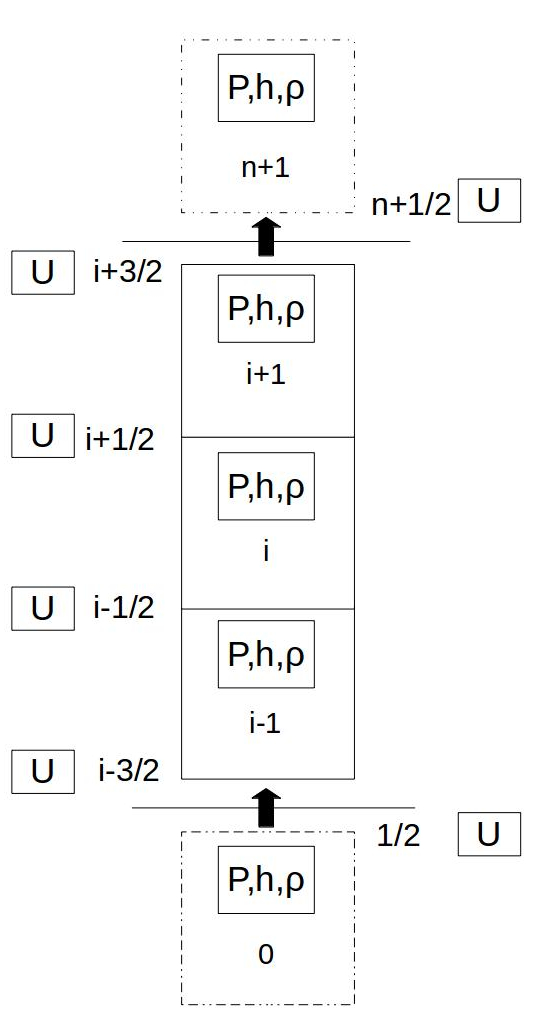
\includegraphics[width=0.30\textwidth]{images/CTF-Cells}
	\caption{The finite volume structure for COBRA-TF}
	\label{fig:CTF-Cells}
\end{figure}

The single phase Euler partial differential equations for mass
\eqref{eq:pde_mass}, momentum \eqref{eq:pde_momentum}, and energy
\eqref{eq:pde_energy} corresond to the unknown variables density $\rho$,
velocity $u$, pressure $P$, and enthalpy $h$. The first terms in each of the
equations are temporal terms. The rest of the terms are steady state spatial
terms. 
    
    \begin{equation}
    	\label{eq:pde_mass}
    	\frac{ \partial \rho}{\partial t} + \bigtriangledown \rho u = 0
    \end{equation}
    
    \begin{equation}
    	\label{eq:pde_momentum}
    	\frac{ \partial \rho u}{\partial t} + \bigtriangledown \rho u^{2} +
    	\bigtriangledown P - \rho g  = 0
    \end{equation}
    
    \begin{equation}
    	\label{eq:pde_energy}
    	\frac{ \partial \rho h}{\partial t} -
    	\frac{ \partial  P}{\partial t} + 
    	\bigtriangledown ( \rho  u h )
    	= 0
    \end{equation}

\subsection{Residual Formulation and Jacobian Construction}

	A residual is simply the difference between the value at some future time
    $n+1$ and the value at the current iteration $k$. This can be applied to
    desired variables and equations. For example, the residual for density,
    $\delta \rho_{i}$, is difference between iterate levels
    $n+1$ and $k$, $\rho^{n+1}_{i} - \rho^{k}_{i}$. The residuals for the
    equations are determined by susbsituting the residuals into the discretized
    equations, which should effectively change all $n+1$ into $k$. Each cell
    will have three residual variables and three residual equations. For the
    entire solution, we will then have a residual variable array $\delta X$, and
    a residual function array $F(X)$ which defines a linear system $J \delta X =
    - F(X)$.
    
    The Jacobian matrix is defined as the derivative
    of each response of the function $F_{j}$ with respect to each variable $X_{i}$.
    The derivative can be calculated numerically as shown by equation
    \eqref{eq:jac_numerical} where $\epsilon$ is a small numerical value. For
    COBRA-TF the equations are linear, and this numerical approximation
    of the Jacobian matrix is exact. This should produce the same jacobian
    matrix that COBRA-TF currently generates analytically. 
    
    \begin{equation}
    	\label{eq:jac_numerical}
    	J_{i,j}=\frac{ \partial F_{j}(X)}{\partial X_{i}}
    	      \approx \frac{F_{j}(X_{i}+\epsilon)-F_{j}(X)}{\epsilon}
    \end{equation}
    
	To build the jacobian matrix, an object oriented class was created that
    contains three arrays. An array that points to the residual functions, an
    array that points to the position within a target variable arrray, and an
    array that has the index that the function is to be evaluated at. These
    lists can be appended to in any order, but have to be appended all at the
    same time so that variables and functions must correspond with each other.
    Then to construct the jacobian matrix, the residual function and residual
    variable arrays can each be looped over to numerically build the jacobian
    matrix as seen in figure \ref{fig:Jacobian_Setup}. 
    
    \begin{figure}[!h]
    	\centering
    	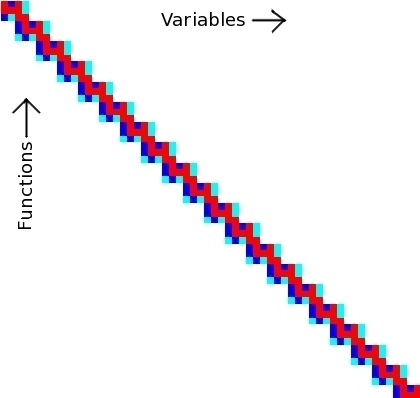
\includegraphics[width=0.40\textwidth]{images/Jacobian_Setup}
    	\caption{Strucutre of the jacobian matrix for single phase liquid}
    	\label{fig:Jacobian_Setup}
    \end{figure}



\section{Isokinetic Sine Wave Advection}

Code verification is the set of procedures set in place to ensure that the code
was written properly. The procedures can use the following as code verification
criteria from least to most rigorous are expert judgement, error quantification,
consistencey / convergence, and order of accuruacy \cite{VV_Book}. For this work
the a Richardson Extrapolation will be used to check for convegence and order of
accruacy of the error in space and time. As shown by the modified equation
analysis in the previous section, the spatial and temporal order of accuracies
should be 1. 
 
\subsection{Problem Setup}

%Round off error, iterative convergence error.
%Discretization error?? (Check with)


The verication problem is defined as a single horizontal channel problem the
base parameters listed in table \ref{table:parameters}. The problem will have a
fixed channel area and perimeter across the entire height of the channel with no
grid spacers. The velocity and pressure are assumed to be constant, but small
fluctuations may occur due to coding mistakes or nuermical noise. The channel
geometry and operating conditions are taken to be approximate a standard PWR.
The inlet of the channel has a constant velocity with a fluctuating enthalpy
that corresponds to a 37.5 $^\circ$C temperature change.  The length
of the transient was defined to be quadrouple the time needed for the liquid at
the inlet to advect to the outlet.The frequencey of the sine wave was defined so
generate a full period of a spatial wave across the height of the channel. 

\begin{table}[h]
\center
\caption{Problem Parameters}
\label{table:parameters}
\begin{tabular}{|c|c|c|c|}
\hline
Parameter	&	Symbol	&	Value	&	Unit	\\ \hline
Axial Height	&	$H$	&	3.6586	&	$m$	\\ \hline
Channel Area	&	$A_{ch}$	&	4.94E-005	&	$m^{2}$	\\ \hline
Wetted Perimeter	&	$P_{w}$	&	1.49E-002	&	$m$	\\ \hline
Velocity	&	$V_{o}$	&	7.35	&	$\frac{m}{s}$	\\ \hline
Pressure	&	$P_{o}$	&	155.00	&	bar	\\ \hline
Temperature 1	&	$T_{1}$	&	289.500	&	$^{\circ}$C	\\ \hline
Temperature 2	&	$T_{2}$	&	327.00	&	$^{\circ}$C	\\ \hline
Enthalpy 1	&	$h_{1}$	&	1281.55	&	$\frac{kJ}{kg}$	\\ \hline
Enthalpy 2	&	$h_{2}$	&	1497.21	&	$\frac{kJ}{kg}$	\\ \hline
Mass Flow Rate 1	&	$\dot{m}_{1}$	&	0.2713	&	$\frac{kg}{s}$	\\ \hline
Mass Flow Rate 2	&	$\dot{m}_{2}$	&	0.2399	&	$\frac{kg}{s}$	\\ \hline
Final Time	&	$t_{f}$	&	2.00	&	sec	\\ \hline
Wave Frequency	&	$\omega$	&	1.00	&	Hz	\\ \hline
\end{tabular}
\end{table}

The lookup table to vary the inlet enthalpy $h$ and inlet mass
flow rate $\dot{m}$ use smooth trigonometric functions given in equations
\ref{eq:Sine_Wave:h} and \ref{eq:Sine_Wave:m_dot}. The equations assume constant
axial spacing $\Delta x$ and time step size $\Delta t$ where $i$ and $j$ are
the spatial and temporal index respectively. These equations should also
behave as the known solutions throughout the entire domain of the problem. The
enthalpy and mass flow rate should vary proportionally to the density as to
create an isokinetic boundary condition at the inlet. However this is dependent
on the steam tables used. A python script was used to generate the data tables
according to trignometric equations using lookup tables that mimic the IAPWS-97
steam tables used by the code \cite{IAPWS}.

\begin{equation}
	\label{eq:Sine_Wave:h}
	h(i,j) = \frac{1}{2} \left( 
			(h_{1}+h_{2}) + (h_{1}-h_{2}) cos\left(
				\omega \left( j \Delta t + \frac{i \Delta x}{V_{o}} \right)
				\right)
			\right)
\end{equation}

\begin{equation}
	\label{eq:Sine_Wave:m_dot}
	\dot{m}(i,j) = \frac{1}{2} \left( 
			(\dot{m}_{1}+\dot{m}_{2}) + (\dot{m}_{1}-\dot{m}_{2}) cos\left(
				\omega \left( j \Delta t + \frac{i \Delta x}{V_{o}} \right)
				\right)
			\right)
\end{equation}


The comparison between the data table and the output in CTF are shown for
enthalpy and mass flow rate in figures \ref{fig:Inlet_h} and
\ref{fig:Inlet_m_dot} respectively. The CTF output was read from hdf5 data files
at each point in time, wich omitted the actual ghost cell where these values
were applied. The CTF values are located at the nearest node to the inlet, and
therefore will be slightly out of phase to the exact values but this effect is
small in the figure.

\begin{figure}[!h]
	\centering
	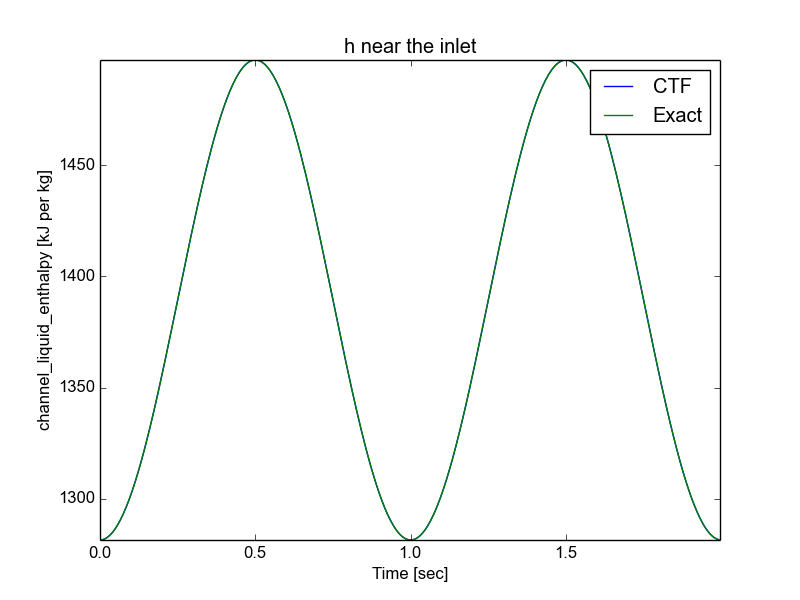
\includegraphics[width=0.55\textwidth]{images/Code_Verification/run_00_00/residual/results/Inlet_h}
	\caption{Enthalpy Near the Inlet and the Analytical Solution}
	\label{fig:Inlet_h}
\end{figure}

\begin{figure}[!h]
	\centering
	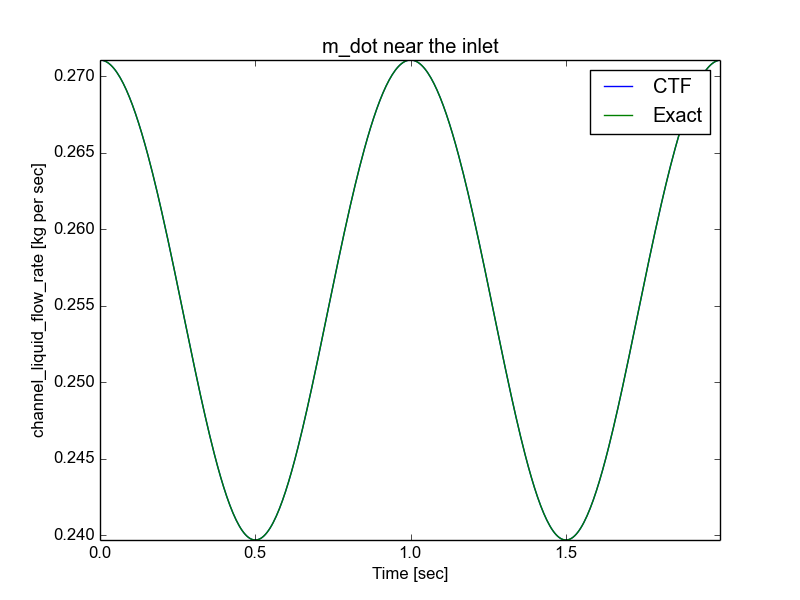
\includegraphics[width=0.55\textwidth]{images/Code_Verification/run_00_00/residual/results/Inlet_m_dot}
	\caption{Density Near the Inlet and the Analytical Solution}
	\label{fig:Inlet_m_dot}
\end{figure}

For the original version of COBRA-TF there is a small discrepancy in the way the
density is calculated at the inlet that causes the velocity to be non-consatnt.
%as shown in figure \ref{fig:Inlet_vel}.
 This is considered small for this problem and should not greatly affect the
 order of accuracy. The residual formulation was coded in such a way as to avoid
 this problem and has considerably less fluctation in the inlet velocity.

\subsection{Code Convergence}

The current version of COBRA-TF uses global code convergance criteria that are
used to estimate the eror assocaited with the solution of the code for transient
and steady state problems as shown in figure
\ref{fig:Code_Convergance:Original}. For this problem, the solid energy storate
is zero since there are not any heat structures present. The fluctuating values
represent differences between the enrgy and mass entering and leaving the
system.

\begin{figure}[!h]
	\centering
	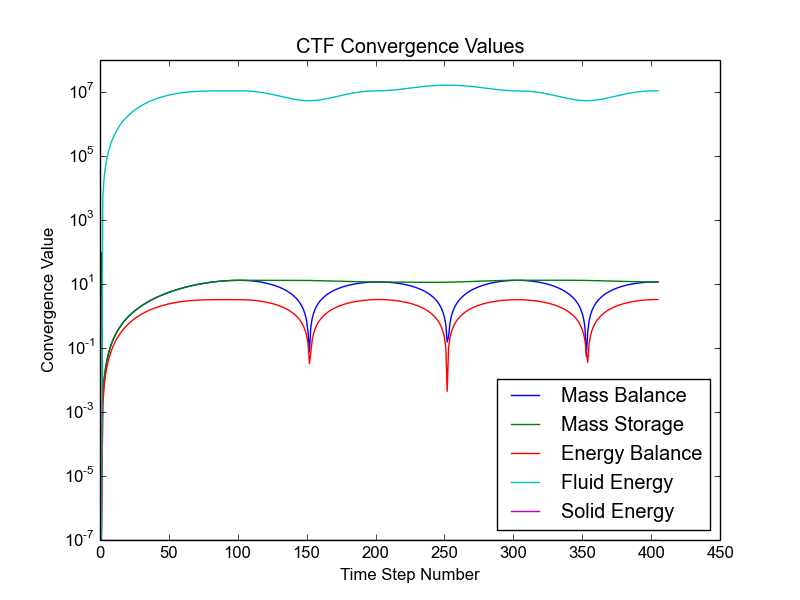
\includegraphics[width=0.50\textwidth]{images/Code_Verification/run_00_00/original/results/Convergence_Plot}
	\caption{Code Convergence Criteria for the original version of COBRA-TF}
	\label{fig:Code_Convergance:Original}
\end{figure}

\begin{figure}[!h]
	\centering
	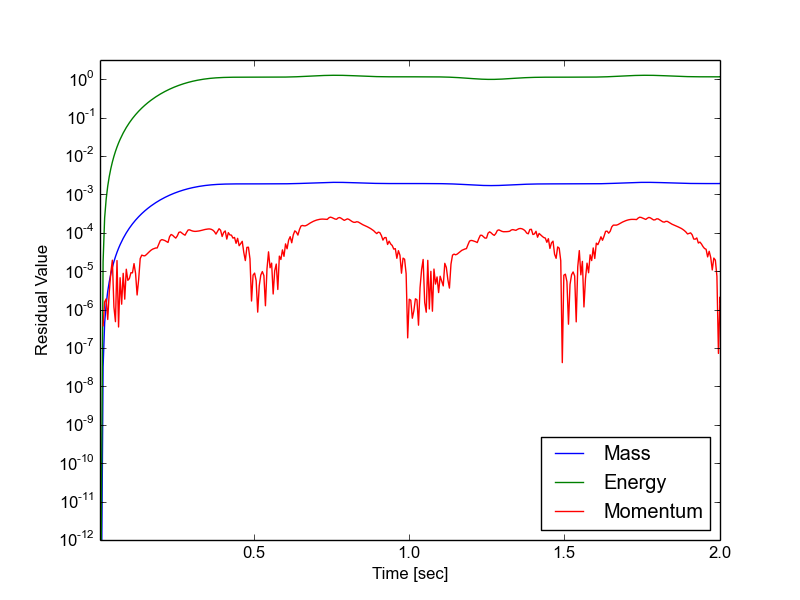
\includegraphics[width=0.50\textwidth]{images/Code_Verification/run_00_00/residual/results/Residuals_Plot}
	\caption{Sumnation of the residuals for the residual version of COBRA-TF}
	\label{fig:Residuals_Plot}
\end{figure}

The residual formulation prints out the sumnation of the residuals functions
across the domain to an output file for eac time step and can be seen in
figure \ref{fig:Residuals_Plot}. The mass balance and energy balances present in
the code convergeance criteria are much smaller for the residual formulation.
These residuals provide a much better indication as to the level of error present in
the solution of the system. They can even be expanded to provide convergence
information at every position, variable, and equation. 



%\subsection{Error Quantification}
%
%\begin{figure}[!h]
%	\centering
%	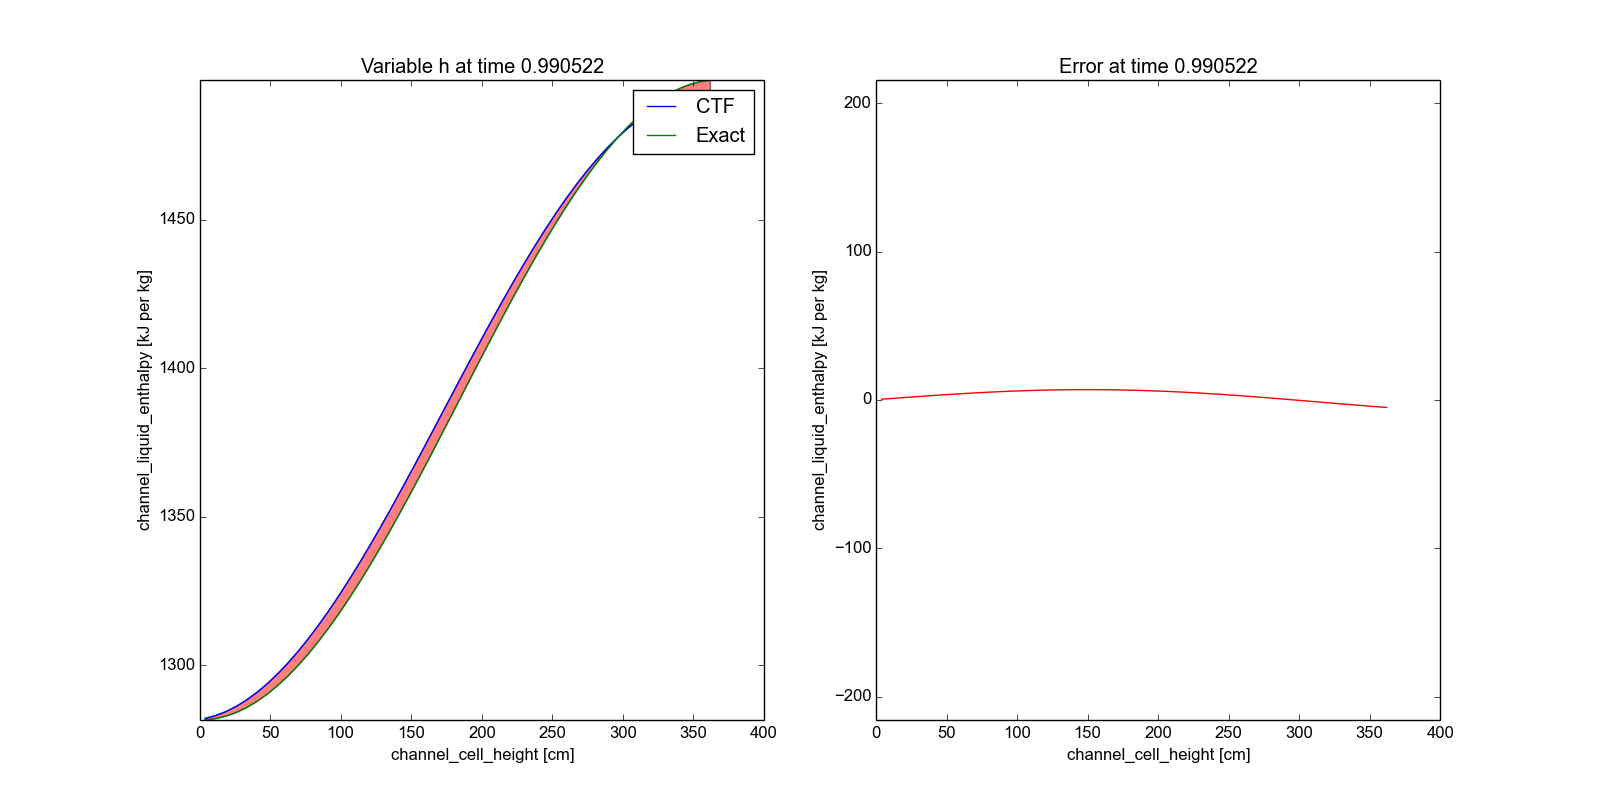
\includegraphics[width=1.00\textwidth]{images/Code_Verification/run_00_01/residual/results/tmp/h_0200.png}
%	\caption{Sumnation of the residuals for the residual version of COBRA-TF}
%	\label{fig:Residuals_Plot}
%\end{figure}
%
%\begin{figure}[!h]
%	\centering
%	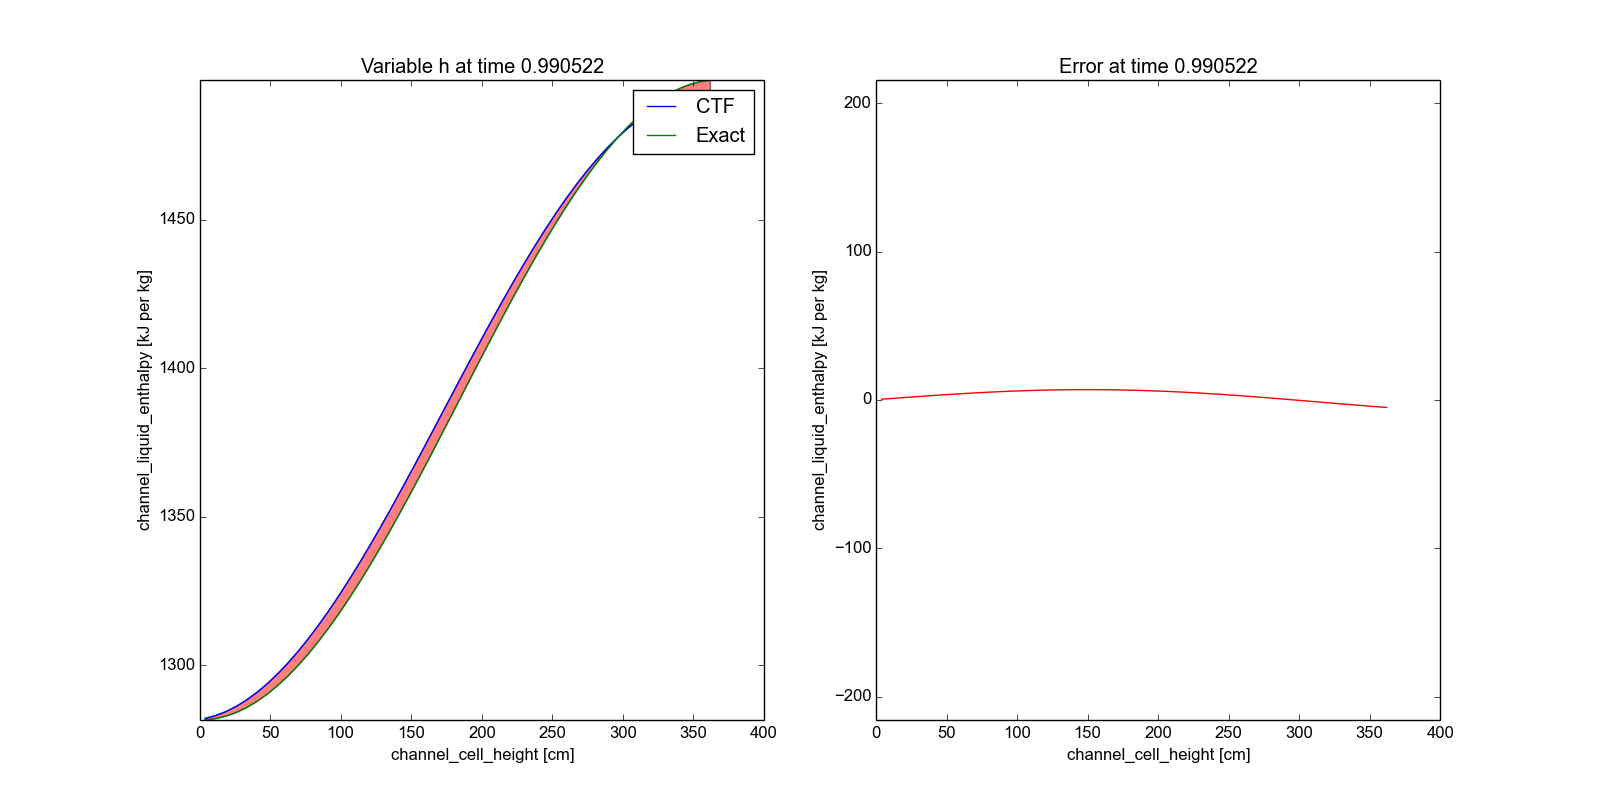
\includegraphics[width=0.55\textwidth]{images/Code_Verification/run_00_01/residual/results/tmp/h_0200}
%	\caption{Sumnation of the residuals for the residual version of COBRA-TF}
%	\label{fig:Residuals_Plot}
%\end{figure}

\subsection{Modified Equation Analysis}
    
    The original mass balance equation can be re-written to 
    look like equation \ref{eq:isokinetic_start}. Using upwinding, the finite difference
    can be written to look like equation \ref{eq:mass_isok_fd}. A second order Taylor 
    series approximation can be used for $\rho_{i}^{n+1}$ and $\rho_{i-1}^{n}$ as shown 
    in equations \ref{eq:rho_taylor_series_time} and \ref{eq:rho_taylor_series_space} 
    respectively. The higher order terms ($O(\Delta x^{2},\Delta t^{2} )$) are
    not taken into account for this approximation. The Taylor series
    approximations can then be substituted into \ref{eq:mass_isok_fd} to yield
    \ref{eq:MEA_start}. This is the beginning of the modified equation analysis.
    The goal will be to isolate the original PDE and define the truncation error.
    
    \begin{equation}
    	\label{eq:isokinetic_start}
    	\frac{\partial \rho}{\partial t} + U_{0} \frac{\partial \rho}{\partial x} = 0
    \end{equation}
    
    \begin{equation}
    	\label{eq:mass_isok_fd}
    	\frac{ \rho_{i}^{n+1} - \rho_{i}^{n} }{\Delta t} 
    	+ U_{0} \frac{\rho_{i}^{n} - \rho_{i-1}^{n}}{\Delta x} = 0
    \end{equation}
    
    \begin{equation}
    	\label{eq:rho_taylor_series_time}
    	\rho_{i}^{n+1} =  \rho_{i}^{n} + 
    	\frac{\partial \rho}{\partial t} \Delta t +
    	\frac{1}{2} \frac{\partial^2 \rho}{\partial t^2} \Delta t^2 + O(\Delta t^{3})
    \end{equation}
    
    \begin{equation}
    	\label{eq:rho_taylor_series_space}
    	\rho_{i-1}^{n} =  \rho_{i}^{n} - 
    	\frac{\partial \rho}{\partial x} \Delta x +
    	\frac{1}{2} \frac{\partial^2 \rho}{\partial x^2} \Delta x^2 + O(\Delta x^{3})
    \end{equation}
    
    The lengthy equation \ref{eq:MEA_start} can be reduced to equation
    \ref{eq:MEA_p0} since the $\rho_{i}^{n}$ terms subtract out and the $\Delta
    t$ and $\Delta x$ terms in the denominator cancel out. This reduced equation
    can the be re-written into equation \ref{eq:MEA_p1}, with the original PDE
    followed by the truncation terms. Notice how the terms on the right are
    dependent on both the numerical spacing $\Delta t$ and $\Delta x$, but also
    on the second derivatives of density with respect to space and time.
    
    \begin{equation}
    	\label{eq:MEA_start}
    	\frac{ \left( \rho_{i}^{n} + \frac{\partial \rho}{\partial t} \Delta t +
    	\frac{1}{2} \frac{\partial^2 \rho}{\partial t^2} \Delta t^2 \right)-\rho_{i}^{n} }{\Delta t} 
    	+ U_{0} \frac{\rho_{i}^{n} - \left( \rho_{i}^{n} -  \frac{\partial \rho}{\partial x} \Delta x + 
    	\frac{1}{2} \frac{\partial^2 \rho}{\partial x^2} \Delta x^2 \right)}{\Delta x} 
    	+ O(\Delta x^{2},\Delta t^{2}) 
    	= 0
    \end{equation}
    
    \begin{equation}
    	\label{eq:MEA_p0}
    	 \frac{\partial \rho}{\partial t}  + \frac{1}{2} \frac{\partial^2 \rho}{\partial t^2} \Delta t +
    	 U_{0} \left(   \frac{\partial \rho}{\partial x}  - \frac{1}{2} \frac{\partial^2 \rho}{\partial x^2} \Delta x \right) 
    	 + O(\Delta x^{2},\Delta t^{2}) 
    	 = 0
    \end{equation}
    
    \begin{equation}
    	\label{eq:MEA_p1}
    	 \frac{\partial \rho}{\partial t}  +  U_{0} \frac{\partial \rho}{\partial x} + 
    	 \frac{1}{2} \frac{\partial^2 \rho}{\partial t^2} \Delta t -
    	   U_{0}  \frac{1}{2} \frac{\partial^2 \rho}{\partial x^2} \Delta x  
    	   + O(\Delta x^{2},\Delta t^{2}) = 0 
    \end{equation} \linebreak
    
%    Before we can procede, we need to take the derivative of the original PDE with respect
%    to space and time as shown in equations \ref{eq:mass_dt} and  \ref{eq:mass_dx} 
%    respectively. These two derivatives can substitute into each other using the common 
%    term $\frac{\partial^2 \rho}{\partial x \partial t}$. The second derivatives of density with 
%    respect to space and time are therefore related by the velocity squared as
%    shown by equation \ref{eq:mass_second_derivatives}.
%    
%    \begin{equation}
%    \label{eq:mass_dt}
%    	 \frac{\partial^2 \rho}{\partial t^2} + U_{0} \frac{\partial^2 \rho}{\partial x \partial t} = 0
%    \end{equation}
%    
%    \begin{equation}
%    \label{eq:mass_dx}
%    	 \frac{\partial^2 \rho}{\partial t \partial x} + U_{0} \frac{\partial^2 \rho}{\partial x^2} = 0
%    \end{equation}
%    
%    \begin{equation}
%    \label{eq:mass_second_derivatives}
%    	 \frac{\partial^2 \rho}{\partial t^2} =  U_{0}^2 \frac{\partial^2 \rho}{\partial x^2}
%    \end{equation} \linebreak
%    
%    This relationship can then be substituted back into equation \ref{eq:MEA_p1}, 
%    which can be reduced to equation \ref{eq:MEA_result} after igonoring the higher
%    order terms. The error depends on the CFL number, the axial spacing, and the
%    second order derivative of density with respect to space. This derivative is
%    what gives the error the characterisitcs of diffusion. When the CFL number is
%    less than one, the error term is negative and the diffusion is dampening. When
%    the CFL number is greater than one, the error term becomes positive, and the
%    accumulation of the error destabilizes the solution. 
%    
%    \begin{equation}
%    	 \frac{\partial \rho}{\partial t}  +  U_{0} \frac{\partial \rho}{\partial x} - 
%    	  \frac{1}{2}  \left(  \Delta x U_{0} \frac{\partial^2 \rho}{\partial
%    	  x^2} -   U_{0}^2 \frac{\partial^2 \rho}{\partial x^2} \Delta t  \right) 
%    	   + O(\Delta x^{2},\Delta t^{2}) = 0
%    \end{equation}
%    
%    \begin{equation}
%    \label{eq:MEA_result}
%    	 \frac{\partial \rho}{\partial t}  +  U_{0} \frac{\partial \rho}{\partial x} - 
%    	 \frac{\Delta x U_{0}}{2} \frac{\partial^2 \rho}{\partial x^2}  
%    	 \left(  1 - CFL  \right) 
%    	 + O(\Delta x^{2},\Delta t^{2})  = 0
%    \end{equation}
%    
%    Modified eqauation analysis can be applied to the energy balance equation
%    presented in equation \ref{eq:MEA_energy}. The energy equation is presented in a form where
%    the momentum equation was substituted in as zero and then divided through by
%    density. The result presented in equation \ref{eq:MEA_ene_result} is similar in
%    form to the result for the mass balance equation \ref{eq:MEA_result}.
%    
%    \begin{equation}
%    	\label{eq:MEA_energy}
%    	\frac{\partial h}{\partial t} - \frac{1}{\rho} \frac{\partial P}{\partial t} +
%    	U_{0} \frac{\partial h}{\partial x} = 0
%    \end{equation}
%    
%    \begin{equation}
%    \label{eq:MEA_ene_result}
%    	\frac{\partial h}{\partial t} - \frac{1}{\rho} \frac{\partial P}{\partial t} +
%    	U_{0} \frac{\partial h}{\partial x} - 
%    	\frac{\Delta x U_{0}}{2} \frac{\partial^2 h}{\partial x^2}
%    	\left( 1 - CFL \right)
%    	= 0
%    \end{equation}

\section{Richardson Extrapolation}

The richardson extrapolation was performed by  refining the spatial and temporal
step sizes by a factor of 2 for a set number of times. The spatial and temporal
studies are refined seperately in their own study in order to isolate the
spatial and temporal affects on the the solution. 


\subsection{Convergence of Error}

The relative difference at each point for a particular time step was calculated
between each iteration for each quantity of interest. For the spatial
refinement, the lower iterate values were numerically integrated to match the
shape of the initial domain. The errors were then sumned over the entire domain
to yield a total error for each variable. The total error for enthalpy is
plotted in figures \ref{fig:Temporal:Diff_h} and \ref{fig:Spatial:Diff_h} as a
function of temporal and spatial step size respecitvely.  The data points where
chosen to be outside of the asymptotic range as shown by the good linear fit of
the data. The plots show that as the temporal and spatial step sizes are
reduced, the numerical error approaches zero. 

\begin{figure}[!h]
	\centering
	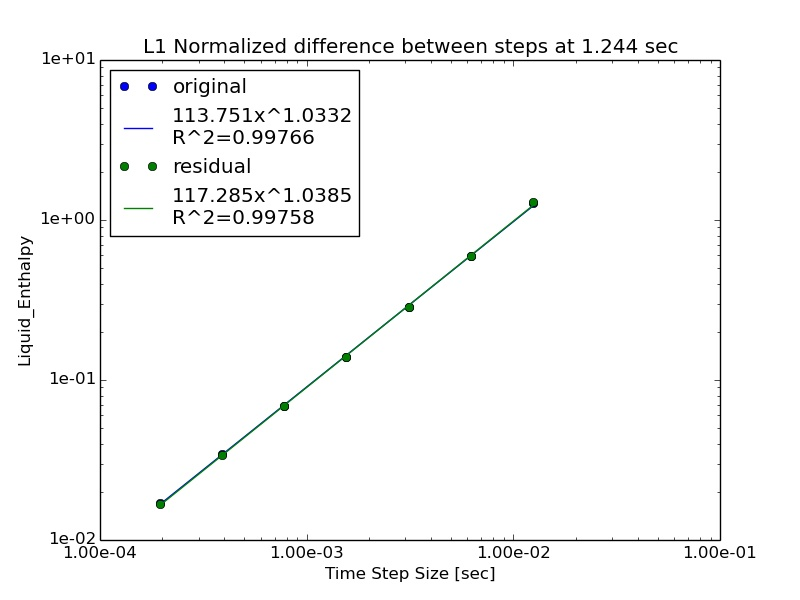
\includegraphics[width=1.00\textwidth]{images/Temporal_Study/Difference_h}
	\caption{Difference Between Succssessive Temporal Refinements}
	\label{fig:Temporal:Diff_h}
\end{figure} 

\begin{figure}[!h]
	\centering
	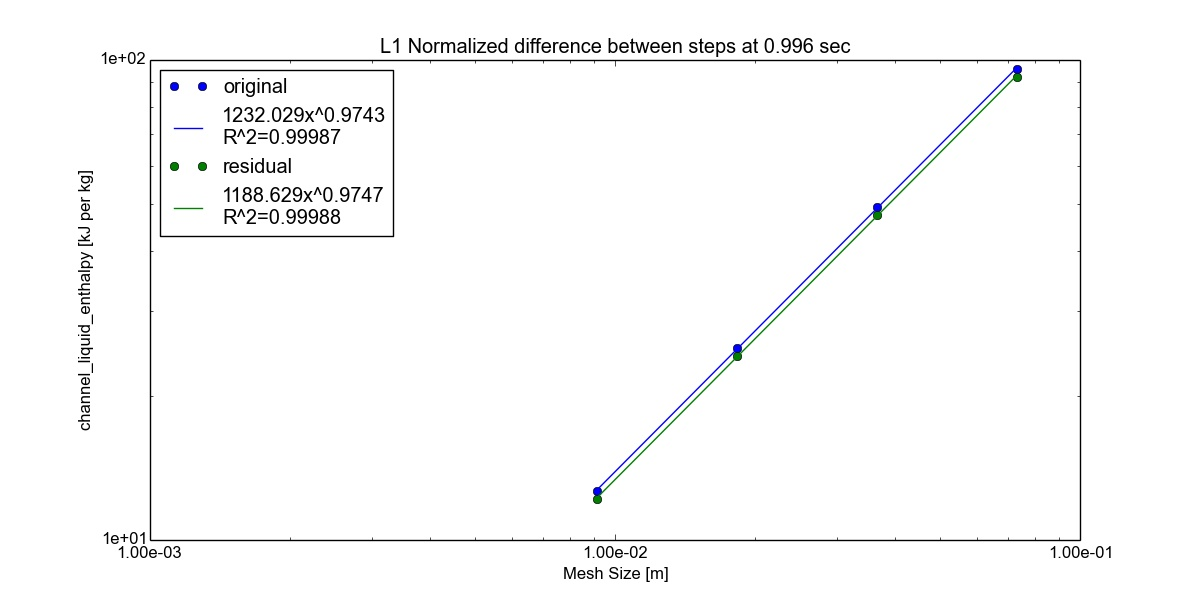
\includegraphics[width=1.00\textwidth]{images/Spatial_Study/Difference_h}
	\caption{Difference Between Succssessive Temporal Refinements}
	\label{fig:Spatial:Diff_h}
\end{figure} 

\subsection{Order of Accuracy}

Each study generates at least 3 points $f_{1}$,$f_{2}$,$f_{3}$ with a constant
refinement factor $R$ of 2. The order of accuracy $p$ between 3 points is given
by equation \eqref{eq:OOA}. 

\begin{equation}
	\label{eq:OOA}
	p= \frac{
	      	ln \left(
	      	\frac{f_{3}-f_{2}}{f_{2}-f_{1}}
	      	\right)
	    }{ln(R)}
\end{equation}

\begin{figure}[!h]
	\centering
	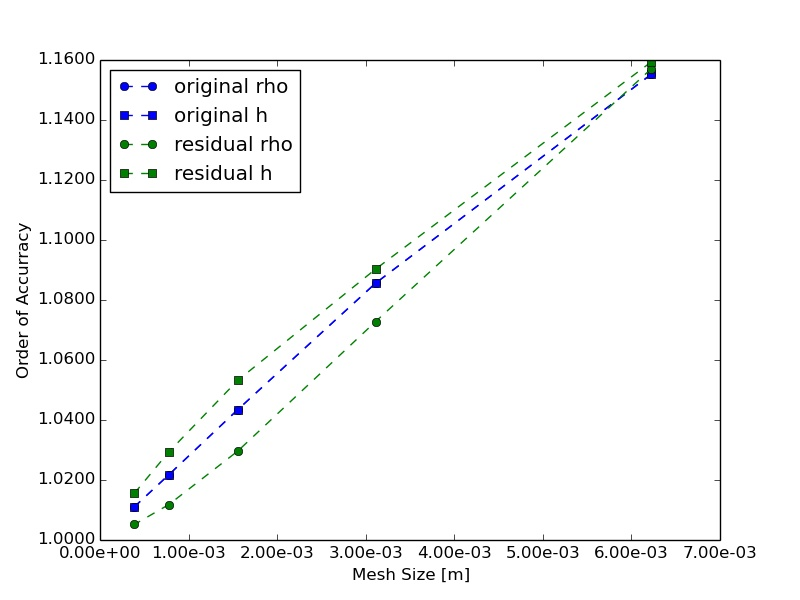
\includegraphics[width=1.00\textwidth]{images/Temporal_Study/Order_Of_Accuracy_Summary}
	\caption{Temporal Order of Accuracy}
	\label{fig:Temporal:OOA}
\end{figure}

\begin{figure}[!h]
	\centering
	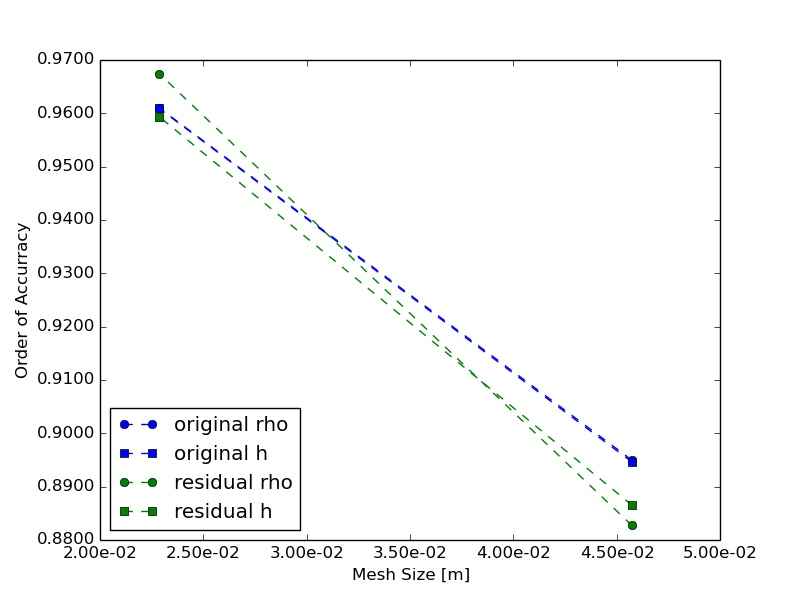
\includegraphics[width=1.00\textwidth]{images/Spatial_Study/Order_Of_Accuracy_Summary}
	\caption{Spatial Order of Accuracy}
	\label{fig:Spatial:OOA}
\end{figure}

%\section{Parameter Study}
%
%Tables and figures of varying the results.
%
%\subsection{Changes in $\Delta$T}
%
%This changes the amplitude of the displacement
%
%\subsection{Changes in Frequencey}
%
%This changes the frequencey of the displacement
%
%\subsection{Changes in Mass Flow Rate}
%
%\section{Computational Time}
%
%The computational time of the two methods for different computational sizes.
%Compare the semi-implicit and fully implicit methods at 0.5 , 1.0, and 2.0 CFL. 

\section{Conclusions}

Present your summary and conclusions here.

\clearpage
%%%%%%%%%%%%%%%%%%%%%%%%%%%%%%%%%%%%%%%%%%%%%%%%%%%%%%%%%%%%%%%%%%%%%
\section{Acknowledgments}

Dr. Vince Mosseau, Dr. Maria Avramova, Dr. Kostadin Ivanov, and Nathan Porter.

%%%%%%%%%%%%%%%%%%%%%%%%%%%%%%%%%%%%%%%%%%%%%%%%%%%%%%%%%%%%%%%%%%%%%
\setlength{\baselineskip}{12pt}

\bibliographystyle{mc2015}
\bibliography{references}

%%%%%%%%%%%%%%%%%%%%%%%%%%%%%%%%%%%%%%%%%%%%%%%%%%%%%%%%%%%%%%%%%%%%%

%\appendix
%\section{}


\end{document}
